\documentclass[tikz,border=2pt]{standalone}
\usepackage{amsmath,amssymb}
\usetikzlibrary{arrows.meta}
\begin{document}
% Cohort counts l_60 = 1000, l_61 = 980, l_65 = 900: d_60 = 20 deaths in the first year,
% q_60 = d_60/l_60 = 0.02 and 5p60 = l_65/l_60 = 0.9 (ratios of table entries).
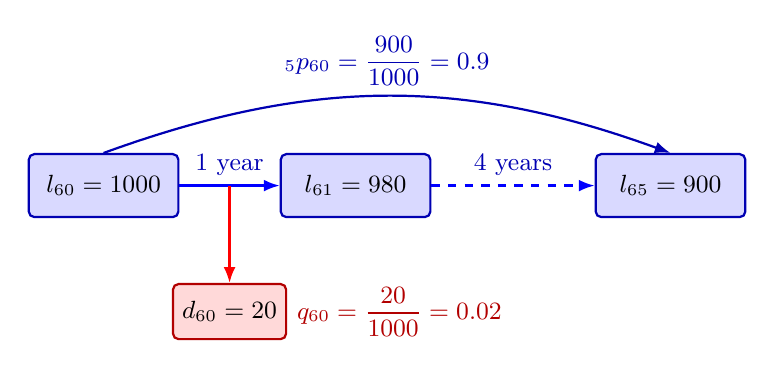
\begin{tikzpicture}[font=\small, >={Latex[length=2mm]},
    box/.style={draw=blue!70!black, thick, fill=blue!15, rounded corners=2pt, minimum width=1.9cm, minimum height=0.8cm}]
  \node[box] (a) at (0,0) {$l_{60}=1000$};
  \node[box] (b) at (3.2,0) {$l_{61}=980$};
  \node[box] (c) at (7.2,0) {$l_{65}=900$};
  \draw[->, blue, thick] (a) -- node[above, blue!70!black] {1 year} (b);
  \draw[->, blue, thick, dashed] (b) -- node[above, blue!70!black] {4 years} (c);
  % deaths
  \node[draw=red!70!black, thick, fill=red!15, rounded corners=2pt, minimum height=0.7cm] (d) at (1.6,-1.6) {$d_{60}=20$};
  \draw[->, red, thick] (1.6,0) -- (d);
  \node[red!70!black, anchor=west] at (d.east) {$q_{60}=\dfrac{20}{1000}=0.02$};
  % 5-year survival
  \draw[->, blue!70!black, thick] (a.north) to[bend left=20] node[above] {${}_5p_{60}=\dfrac{900}{1000}=0.9$} (c.north);
\end{tikzpicture}
\end{document}
